\section{Computing time bounds}

This chapter presents a method, which is able to infer time bounds for the transitions of a program.
The original KoAT paper \cite{koat} presents two approaches: One basic approach, which considers the whole program at once and a modular approach, which considers a selected subset of the program transitions.
This master's thesis only considers the modular approach since the other approach can be defined as a special case of the modular approach.

The presented method is based on ranking functions.
The original KoAT allows the usage of polynomial ranking functions.
It uses an operator on the polynomials, which considers the absolute values of variables and converts all negative signs into positive signs.
This is necessary to ensure component-wise monotonicity of the variables in the polynomials.
Otherwise, a substitution of the variables with the size bounds would not necessarily be a sound overapproximation.
The new method does not use this operator.
Instead, the presented approximated replacement is used, which chooses the appropriate upper and lower size bound for the substitution of a variable with respect to its monotonicity in the ranking polynomial.
As already mentioned, this approach is the more effective, the more we know about the monotonicity about the variables.
Considering affine polynomials yields the best results since in an affine polynomial every variable is either monotonically increasing or monotonically decreasing.
In practice most existing techniques generate these affine ranking functions (e.g. \cite{podelski2004prf}, \cite{bradley2005linear}, \cite{bagnara2012new}, \cite{leike2014ranking}, \cite{ben2013linear}).
But in general, the new method is also applicable to polynomial ranking functions.

For the definition of the method, we need to define the terms of entry locations and entry transitions.
\begin{definition}[Entry transitions and entry locations]
  Let $\TSet' \subseteq \TSet$ be a nonempty subset of all transitions.
  We define the entry transitions $\TSet_{\location}$ of a location $\location$ as $\braced{(\location', \update, \guard, \location) \mid \exists \location', \update, \guard: (\location', \update, \guard, \location) \in \TSet \setminus \TSet'}$.
  We define the entry locations $\mathcal{E}_{\TSet'}$ of the transition set $\TSet'$ as $\braced{\location_{in} \mid \TSet_{\location_{in}} \neq \emptyset \wedge \exists \location': (\location_{in}, \update, \guard, \location') \in \TSet'}$.
\end{definition}
This is the same definition used in the original KoAT paper \cite{koat}.

\begin{example}[Entry transitions and entry locations]
  \begin{figure}
\centering
\begin{tikzpicture}[->,>=stealth',auto,node distance=3cm,
    thick,
    main node/.style={circle,draw,font=\sffamily\Large\bfseries},
    aligned edge/.style={align=left}]

  \node[main node] (0) {$l_0$};
  \node[main node] (1) [right of=0] {$l_1$};
  \node[main node] (2) [right of=1] {$l_2$};
  \node[main node] (3) [right of=2] {$l_3$};

  \path[every node/.style={font=\sffamily\small}]
    (0) edge[aligned edge] node[above=0.2cm] {$t_0$} (1)
    (1) edge[aligned edge, loop above] node[above=0.2cm] {$t_1$} (1)
    (1) edge[aligned edge] node[above=0.2cm] {$t_2$} (2)
    (2) edge[aligned edge, bend left] node[above=0.2cm] {$t_3$} (3)
    (3) edge[aligned edge, bend left] node[below=0.2cm] {$t_4$} (2)
    ;
\end{tikzpicture}
\begin{tikzpicture}[->,>=stealth',auto,node distance=3cm,
    thick,
    main node/.style={circle,draw,font=\sffamily\Large\bfseries},
    aligned edge/.style={align=left}]

  \node[main node] (0) {$l_0$};
  \node[main node, dotted] (1) [right of=0] {$l_1$};
  \node[main node, dotted] (2) [right of=1] {$l_2$};
  \node[main node] (3) [right of=2] {$l_3$};

  \path[every node/.style={font=\sffamily\small}]
    (0) edge[aligned edge] node[above=0.2cm] {$t_0$} (1)
    (1) edge[aligned edge, ultra thick, loop above] node[above=0.2cm] {$t_1$} (1)
    (1) edge[aligned edge] node[above=0.2cm] {$t_2$} (2)
    (2) edge[aligned edge, ultra thick, bend left] node[above=0.2cm] {$t_3$} (3)
    (3) edge[aligned edge, ultra thick, bend left] node[below=0.2cm] {$t_4$} (2)
    ;
\end{tikzpicture}
\caption{A program for showing the difficulties of chosing the right subset of transitions}
\label{fig:entrytransitions}
\end{figure}

  As an example, consider the programs in Figure \ref{fig:entrytransitions}.
  In each of the programs, a chosen set $\TSet' \subseteq \TSet$ is highlighted with bold arrows.
  Additionally, all entry locations and entry transitions are shown with dashed arrows.
  In the first program, the set of transitions $\TSet' = \braced{t_1, t_3, t_4}$ does have two entry locations $\mathcal{E}_{\TSet'} = \braced{\location_1, \location_2}$.
  These entry locations define the entry transitions $\TSet_{\location_1} = \braced{t_0}$ and $\TSet_{\location_2} = \braced{t_2}$.
  The second program only has one entry location $\mathcal{E}_{\TSet'} = \braced{\location_1}$ and therefore only one entry transition $\TSet_{\location_1} = \braced{t_0}$.
  The third program also has just one entry location, but in this example it is $\mathcal{E}_{\TSet'} = \braced{\location_2}$.
  Its entry transition is $\TSet_{\location_2} = \braced{t_2}$.
\end{example}

Now it is possible to define the method for the construction of time bounds.

\begin{theorem}[TimeBounds]
  Let $(\UTime, \Size)$ be a complexity approximation. \\
  Let $\TSet' \subseteq \TSet \setminus \TSet_0$ a subset of all transitions such that $\TSet'$ contains no initial transitions. \\
  Let $\TSet_{\location} = \braced{(\location', \update, \guard, \location) \mid \exists \location', \update, \guard: (\location', \update, \guard, \location) \in \TSet \setminus \TSet'}$ denote the set of all transitions outside of the subprogram $\TSet'$ leading to an $\location \in \LSet$. \\
  Let $\mathcal{E}_{\TSet'} = \braced{\location_{in} \mid \TSet_{\location_{in}} \neq \emptyset \wedge \exists \location': (\location_{in}, \update, \guard, \location') \in \TSet'}$ denote the set of all entry locations of $\TSet'$. \\
  Let $\timerank: \LSet \rightarrow \BoundSet_a(\PVSet)$ be an \textbf{affine} time ranking function for $\TSet'$. \\
  For $t \in \TSet'_>$ let
  \[ \UTime'(t) = \sum_{\location \in \mathcal{E}_{\TSet'}} \sum_{\pret \in \TSet_\location} \UTime(\pret) \cdot \maxO{\usubst{\timerank(\location)}{\LSize(\pret)}{\USize(\pret)}} \]
  Let $\UTime'(t) = \UTime(t)$ for $t \in \TSet \setminus \TSet'_>$. \\
  Then, $\text{TimeBounds}(\UTime, (\USize, \LSize), \TSet') = \UTime'$ is also a runtime approximation.
\end{theorem}


The idea of this method is, that a time rank $\timerank(\location)$ of an entry location $\location \in \mathcal{E}_{\TSet'}$ is a time bound for all decreasing transitions $t \in \TSet'_>$ depending on the values of the variables at the location $\location$.
If we lift this time bound, such that it depends on the values of the variables at the start location $\location_0$ of the program, we obtain a global time bound.
For this purpose, we first need to substitute all variables of the time rank $\timerank(\location)$ with the size bounds $\USize(r), \LSize(r)$ from the start location $\location_0$ to the transition $r \in \TSet_{\location}$ immediately before the location $\location$.
By definition of the approximated replacement, a substitution $\usubst{\timerank(\location)}{\LSize(r)}{\USize(r)}$ results in such a bound while it ensures, that the result is still an overapproximation. 
Since a time bound shall only be positive, we apply a $\maxO{\cdot}$ operator to the result $\usubst{\timerank(\location)}{\LSize(r)}{\USize(r)}$.
Now, we have to overapproximate the number of evaluations which might enter through the entry location $\location$.
The previous time bound $\UTime$ yields such a bound for all entry transitions.
Then, $\sum_{\location \in \mathcal{E}_{\TSet'}} \sum_{\pret \in \TSet_\location} \UTime(\pret) \cdot \maxO{\usubst{\timerank(\location)}{\LSize(\pret)}{\USize(\pret)}}$ is a time bound for each strictly decreasing transition $t \in \TSet'_>$ depending on the values of the variables from the start.

\begin{example}[TimeBounds]
  \begin{figure}
  \centering
  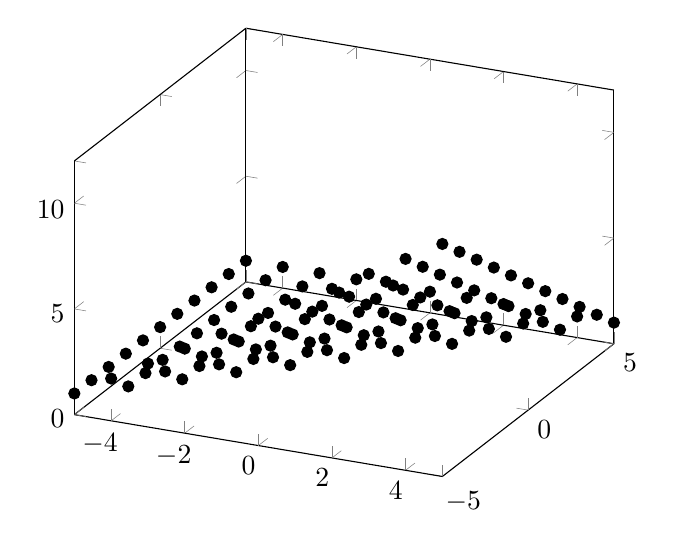
\begin{tikzpicture}
    \begin{axis}
      \addplot3 [
        unbounded coords=jump,
        mesh,
        shader=interp,
        samples at={-5,...,5},
        samples y={11},
        only marks,
      ] {1+max(x-y,0)};
    \end{axis}
  \end{tikzpicture}
  \hfil
  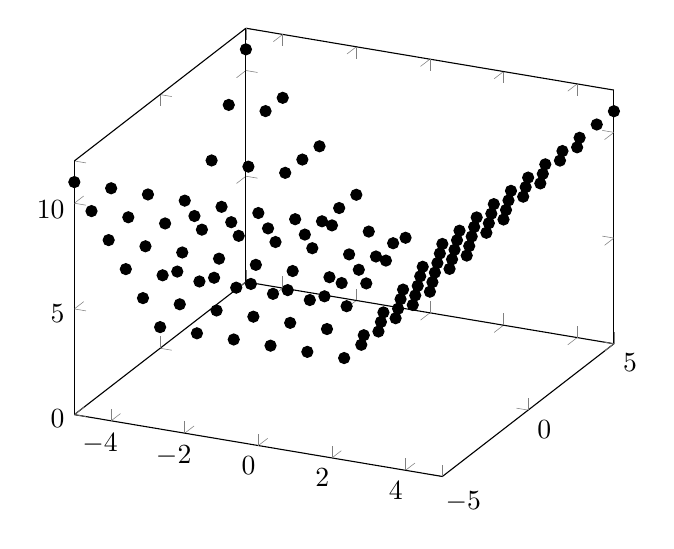
\begin{tikzpicture}
    \begin{axis}
      \addplot3 [
        unbounded coords=jump,
        mesh,
        shader=interp,
        samples at={-5,...,5},
        samples y={11},
        only marks,
      ] {1+abs(max(x,-y))+abs(max(x,-y))};
    \end{axis}
  \end{tikzpicture}
  \caption{Evaluation of the motivational example}
  \label{fig:motivational_evaluation}
\end{figure}

  As an example, we consider the motivational program in Figure \ref{fig:motivational_example} from the introduction.
  With the transition set $\TSet' = \braced{t_1}$ it is possible to determine a ranking function $\timerank(\location_1) = x - y$, since the transition $t_1$ decreases the measure and no transition increases the measure (since no other transition exists in $\TSet'$).
  The original KoAT would now apply an operator to $\timerank$, such that the result would be a monotonic function with $\timerank'(\location_1) = \abs{x} + \abs{y}$.
  Then, it is able to substitute each variable by its absolute size bound and therefore lift it to a global context.
  The new method does not use this operator.
  Instead, it substitutes each variable of $\timerank(\location_1)$ by its lower/upper size bound depending on the monotonicity of the variables in the time rank.
  Since $x$ is monotonically increasing in $x-y$ and $y$ is monotonically decreasing in $x-y$, we can substitute $x$ with the upper size bound and $y$ with the lower size bound.
  Lets assume, that we already inferred the size bounds $\USize(t_0,x) = \LSize(t_0,x) = x$ and $\USize(t_0,y) = \LSize(t_0,y) = y$.
  It is now possible to lift the components of the ranking functions to a global level.
  \[ \usubst{\timerank(\location)}{\LSize(t_0)}{\USize(t_0)} = \USize(t_0, x) - \LSize(t_0, y) = x - y \]
  Note that with a state $\valuation$ with $\valuation(x) < \valuation(y)$ the transition $t_1$ will simply not occur in an evaluation instead of occurring a negative number of times.
  To reflect this in the new time bound, we have to ensure the positivity of $x - y$ with the operation $\maxO{x - y}$.
  Then, the only step left is to consider the number of times an evaluation might enter the SCC from $t_0$.
  Since $t_0$ is an initial transition, its time bound is $\UTime(t_0) = 1$.
  Therefore, an evaluation might only enter a single time from $t_0$ and the resulting time bound for $t_1$ is $\maxO{x - y}$.
\end{example}

The choice of the transition set $\TSet'$ has a major impact on the quality of the time bounds.
Consider again the three programs in Figure \ref{fig:entrytransitions}.

A trivial choice for $\TSet'$ would be all non-initial transitions.
This choice is shown in the second program with $\TSet' = \TSet \setminus \TSet_0 = \braced{t_1, t_2, t_3, t_4}$.
For this choice we have entry locations $\mathcal{E}_{\TSet'} = \braced{\location_1}$ and entry transitions $\TSet_{\location_1} = \braced{t_0}$.
Therefore, for each transition $t \in \TSet'_>$ we end up with $\UTime'(t) = \UTime(t_0) \cdot \maxO{\usubst{\timerank(\location_1)}{\LSize(t_0)}{\USize(t_0)}}$.
Since $t_0 \in \TSet_0$ is an initial transition, we have $\UTime(t_0) = 1$ and therefore $\UTime'(t) = \maxO{\usubst{\timerank(\location_0)}{\LSize(t_0)}{\USize(t_0)}}$ for all transitions $t \in \TSet'_>$.

This trivial choice requires finding a ranking function, that satisfies the non-increasing constraint for all transitions of the program.
If no such ranking function can be found, it is impossible to infer any time bounds with this choice of the transition set $\TSet'$.
But since the method allows us to consider a subset of these transitions, it might be possible, to remove the transition which violates its non-increasing constraint.
Then, a ranking function may be found.

Assume that the transition violating the non-increasing constraint is $t_1$ and consider the third example in Figure \ref{fig:entrytransitions} with the choice $\TSet' = \braced{t_3, t_4}$.
Since the transition set is smaller, there are fewer constraints and it is more likely to find a ranking function.
For the transition set $\TSet' = \braced{t_3, t_4}$, we have the entry locations $\mathcal{E}_{\TSet'} = \braced{\location_2}$ and the entry transitions $\TSet_{\location_2} = \braced{t_2}$.
Since the transition $t_2$ is not part of a loop, its time bound is $\UTime(t_2) = 1$.
Therefore, we end up with $\UTime'(t) = \maxO{\usubst{\timerank(\location_2)}{\LSize(t_2)}{\USize(t_2)}}$.

Note that the subset of transitions $\TSet' \subseteq \TSet$ does not need to be strongly connected.
For example, a subset consisting of two SCCs $\TSet' = \braced{t_1, t_3, t_4}$ can be chosen.
This choice leads to a time bound $\UTime'(t) = \maxO{\usubst{\timerank(\location_1)}{\LSize(t_0)}{\USize(t_0)}} + \maxO{\usubst{\timerank(\location_2)}{\LSize(t_2)}{\USize(t_2)}}$.
This is a valid time bound for transitions $t \in \TSet'_>$.
But two independent analyses for the SCCs $\braced{t_1}$ and $\braced{t_3, t_4}$ could yield time bounds $\UTime'(t) = \maxO{\usubst{\timerank(\location_1)}{\LSize(t_0)}{\USize(t_0)}}$ for the first SCC and $\UTime'(t) = \maxO{\usubst{\timerank(\location_2)}{\LSize(t_2)}{\USize(t_2)}}$ for the second SCC, since each analysis would now consider its own entry locations $\location_1$ and $\location_2$.

Also, only a part of an SCC such as $\TSet' = \braced{t_4}$ could be chosen.
But since the transition $t_3 \in \TSet_{\location_3}$ is an entry transition of $\TSet' = \braced{t_4}$, this only results in a non-trivial time bound $\neq \infty$, if there already exists a time bound $\UTime(t_3) < \infty$ for the transition $t_3$.
Even if there is a time bound $\UTime(t_3) < \infty$, the consideration of the transition $t_3$ as entry transition yields an additional addend for the new time bound $\UTime(t_4)$.
If the found ranking function guarantees that $t_3$ is a non-increasing transition, it would not be necessary to consider it as an entry transition and therefore the new time bound $\UTime(t_4)$ would be reduced.

These examples show, that the best choice of a transition set $\TSet'$ is not trivial.
The implementation uses a backtracking algorithm, which analyses each SCC independently, and considers multiple selections of transition sets to reduce the number of entry transitions.
